% Copyright (c) 2020, Santtu Söderholm <santtu.soderholm@tuni.fi>
%
% This file may be distributed and/or modified under the LaTeX Project Public License.
%

\begin{frame}[noframenumbering, plain]
\titlepage
\end{frame}

\begin{frame}[noframenumbering, plain]{Table of contents}
\tableofcontents
\end{frame}

\section{Components needed for inference}
\begin{frame}{Components needed for inference}
\begin{table}[ht]
\centering
\begin{tabular}{|l|p{8cm}|}
\hline
\textbf{Item} & \textbf{Description} \\ \hline
Platform & SocHub's Headsail SoC with a Deep Learning Accelerator. Development done in a virtual prototype. \\ \hline
Compiler & riscv64-unknown-none-elf. \\ \hline
BSP (Board Support Package) & Support for necessary hardware peripherals. \\ \hline
Machine Learning Compiler & Convert high-level models to Headsail compatible code. \\ \hline
Model & 3 MLPerf Tiny reference models \\ \hline
Dataset &  3 datasets defined by MLPerf Tiny benchmark  \\ \hline
\end{tabular}
\caption{System Configuration and Components}
\label{tab:system_components}
\end{table}
\end{frame}

\section{Headsail}
\begin{frame}{SoCHub Headsail}
  \begin{itemize}
          \item RISC-V based SoC developed at Tampere University
          \item 4-core multicore CPU in HPC
          \item Deep Learning Accelerator for CNNs
          \item Large SDRAM for Data ( 128MB )
  \end{itemize}
  Goal: Build software stack for the DLA to support inference on arbitrary convolutional models

\end{frame}

\section{DLA}
\begin{frame}{DLA}
    \begin{columns}

        \begin{column}{0.4\textwidth}
          \begin{itemize}
                  \item Supported operations are Conv2D, Bias and ReLU
                  \item Arithmetic width of 16 bits, results 8 bits signed
                  \item Input from internal buffer accessible from anywhere in the SoC
                  \item Operation parameters defined in register interface
          \end{itemize}
        \end{column}

        \begin{column}{0.6\textwidth}
            \begin{figure}
                \vfill
                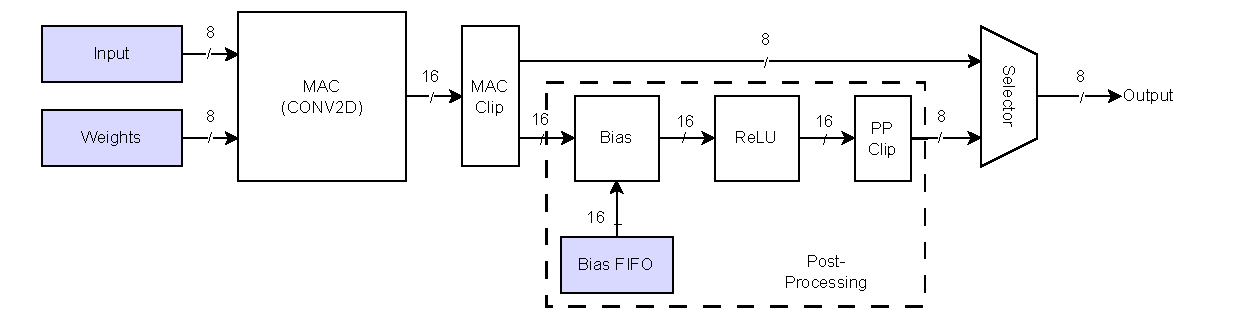
\includegraphics[width=1.0\textwidth]{../../thesis/img/dla-internal.pdf}
                \caption{projects software architecture}
            \end{figure}
        \end{column}
    \end{columns}
\end{frame}

\begin{frame}{DLA}
\begin{columns}
    \begin{column}{0.5\textwidth}
      \begin{itemize}
              \item HPC (RV64) controls DLA with the register interdace
              \item DLA internal databanks filled with data from SDRAM
              \item 64 and 32-bit AXI buses enable fast data transfers
              \item DLA writes results to data banks or directly back to SDRAM
      \end{itemize}
      \end{column}
    \begin{column}{0.5\textwidth}
  \begin{figure}
    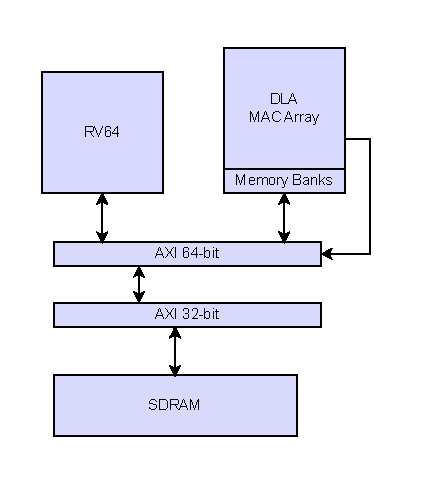
\includegraphics[width=0.7\textwidth]{../../thesis/img/dla-setup.drawio.pdf}
    \caption{Projects software architecture}
  \end{figure}
    \end{column}
\end{columns}
\end{frame}

\section{TVM}
\begin{frame}{TVM}
  \begin{itemize}
          \item Open-source Machine Learning Compiler that supports large variety of hardware backends~\cite{TVM}
          \item BYOC offers a way to integrate custom accelerators to TVM
          \item Runtime for bare-metal targets via microTVM, dependent only on C standard library
          \item Custom legalization pass performs graph transformation to support custom hardware targets
  \end{itemize}
\end{frame}

\section{MLPerf Tiny}
\begin{frame}{MLPerf Tiny}
\begin{table}[ht]
\centering
\caption{Tiny Performance Benchmarks, from~\parencite{tinyperf}}
\begin{adjustbox}{max width=\textwidth}
\begin{tabular}{lccc}
  \toprule
  \textbf{Benchmark} & \textbf{Dataset (Input Size)} & \textbf{Model (TFLite Model Size)} & \textbf{Quality Target (Metric)} \\
  \midrule
  Keyword Spotting & Speech Commands (49x10) & DS-CNN (52.5 KB) & 90\% (Top-1) \\
  Visual Wake Words & VWW Dataset (96x96)  & MobileNetV1 (325 KB) & 80\% (Top-1) \\
  Image Classification & CIFAR10 (32x32) & ResNet (96 KB) & 85\% (Top-1) \\
  Anomaly Detection & ToyADMOS (5x128)  & FC-AutoEncoder (270 KB) & .85 (AUC) \\
  \bottomrule
\end{tabular}
\end{adjustbox}
\label{tab:tinyperf}
\end{table}
\end{frame}

\section{Software Acrchitecture}
\begin{frame}{Final software architecture}
  \begin{figure}
    \vfill
    \hfill
    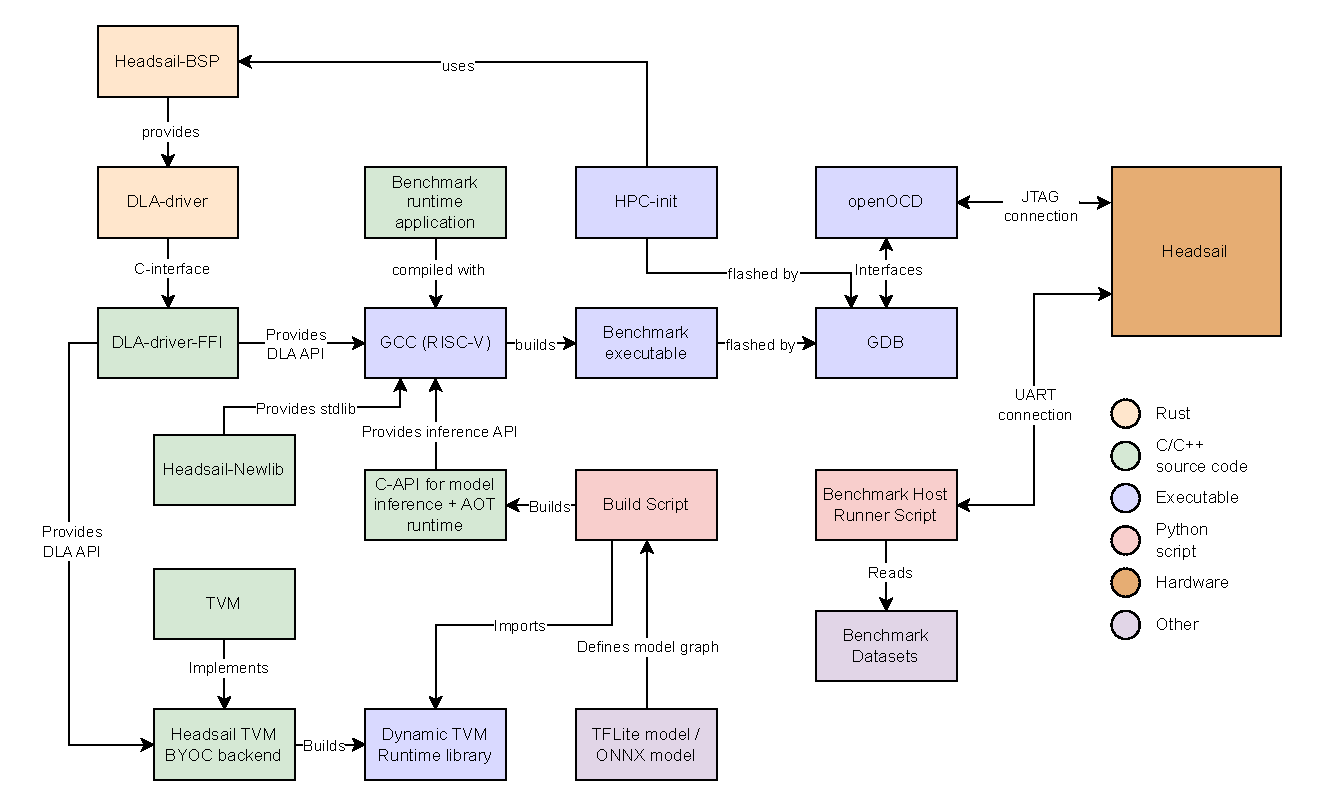
\includegraphics[height=0.6\textheight]{../../thesis/img/dla-architecture-new.pdf}
    \caption{Projects software architecture}
  \end{figure}
\end{frame}

\section{Results}
\begin{frame}{Results}
\begin{table}[h]
\centering
\begin{tabular}{|l|l|c|c|c|c|}
\hline
  \multirow{2}{*}{\textbf{Task}}  & \multirow{2}{*}{\textbf{Target}}  & \multirow{2}{*}{\textbf{Accuracy}} & \multirow{2}{*}{\textbf{Precision}} & \multirow{2}{*}{\textbf{Recall}} & \multirow{2}{*}{\shortstack[c]{\textbf{Passes}\\ \textbf{MLPerf Tiny}}} \\
  & & & & & \\\hline
\multirow{2}{*}{\shortstack[l]{\textbf{Keyword}\\ \textbf{Spotting (KWS)}}}
                                  & \textbf{HPC} & 0.90               & 0.92       & 0.90     & Yes                          \\ \cline{2-6}
                                  & \textbf{HPC+DLA} & 0.90               & 0.92   & 0.90         & Yes                          \\ \hline
\multirow{2}{*}{\shortstack[l]{\textbf{Image}\\ \textbf{Classifcation (IC)}}}
                                  & \textbf{HPC} & 0.88               & 0.88      & 0.88      & Yes                          \\ \cline{2-6}
                                  & \textbf{HPC+DLA} & 0.69               & 0.74      & 0.70      & No                           \\ \hline
\multirow{2}{*}{\shortstack[l]{\textbf{Visual Wake}\\ \textbf{Words (VWW)}}}
                                  & \textbf{HPC} & 0.83               & 0.83        & 0.84    & Yes                          \\ \cline{2-6}
                                  & \textbf{HPC+DLA} & 0.50               & 0.50   & 0.50          & No                           \\ \hline
\multirow{2}{*}{\shortstack[l]{\textbf{Anomaly}\\ \textbf{Detection (AD)}}}
                                  & \textbf{HPC} & -               & -        & -    & Yes                          \\ \cline{2-6}
                                  & \textbf{HPC+DLA} & -               & -   & -          & No                           \\ \hline

\end{tabular}
\caption{MLPerf Tiny benchmark results for HPC and HPC with DLA.}
\label{tab:benchmark-results}
\end{table}
\end{frame}
\section{References}

\begin{frame}{References}
    \printbibliography[heading=none]
\end{frame}

\finalpage{Thank you for listening!}{Questions?}
